\lab{Dynamic Programming}{Dynamic Programming}
\objective{Sequential decision making problems are a class of problems in which the current choice depends on future choices.
They are a subset of Markov decision processes, an important class of problems with applications in business, robotics, and economics.
Dynamic programming is a method of solving these problems that optimizes the solution by breaking the problem down into steps and optimizing the decision at each time period.
In this lab, we use dynamic programming to solve two classic dynamic optimization problems.}

\section*{The Marriage Problem} % =============================================

Many dynamic optimization problems can be classified as \emph{optimal stopping} problems, where the goal is to determine at what time to take an action to maximize the expected reward.
For example, when hiring a secretary, how many people should you interview before hiring the current interviewer?
Or how many people should you date before you get married?
These problems try to determine at what person $t$ to stop in order to maximize the chance of getting the best candidate.

For instance, let $N$ be the number of people you could date.
After dating each person, you can either marry them or move on; you can't resume a relationship once it ends.
In addition, you can rank your current relationship to all of the previous options, but not to future ones.
The goal is to find the policy that maximizes the probability of choosing the best marriage partner.
That policy may not always choose the best candidate, but it should get an almost-best candidate most of the time.

Let $V(t-1)$ be the probability that we choose the best partner when we have passed over the first $t-1$ candidates with an optimal policy.
By Bellman's optimality equations,
\begin{equation}
\label{eq:dynamicopt-do7}
V(t-1) = \frac{t-1}{t}V(t)+\frac{1}{t}\max\left\{ \frac{t}{N},V(t)\right\} = \max\left\{\frac{t-1}{t}V(t)+\frac{1}{N},V(t)\right\}.
\end{equation}

That is, $V(t-1)$ is split into two possibilities.
When candidate $t$ is not the best so far, we use the left-hand side of the last equation, $\frac{t-1}{t}V(t)+\frac{1}{N}$.
Unless this is the last candidate, we don't want to choose them because we've seen someone better.
When candidate $t$ is the best so far, we use the right-hand side, $V(t)$.
We can either choose this candidate, in which case they turn out to be the best match with probability $\frac{t}{N}$, or move on.
Notice that \eqref{eq:dynamicopt-do7} implies that $V(t-1)\geq V(t)$ for all $t\leq N$.
Hence, the probability of selecting the best match $V(t)$ is non-increasing.
Conversely, the probability that if candidate $t$ is the best so far, then they are also the best overall, $\frac{t}{N}$, is strictly increasing.
Therefore, there is some $t_0$, called the \emph{optimal stopping point}, such that $V(t)\leq\frac{t}{N}$ for all $t\geq t_0$.
After $t_0$ relationships, we choose the next partner who is better than all of the previous ones.
We can write \eqref{eq:dynamicopt-do7} as
\[
V(t-1) =
    \begin{cases}
    V(t_0) & t<t_0,\\
    \frac{t-1}{t}V(t)+\frac{1}{N} & t\geq t_0.\\
    \end{cases}
\]

The goal of an optimal stopping problem is to find $t_0$, which we can do by backwards induction on the second piece of $V(t-1)$.
We start at the final candidate, who always has probability $0$ of being the best overall if they are not the best so far, and work our way backwards, computing the expected value $V(t)$, for $t=N,N-1,\ldots,1$.
Notice that the first candidate is always the best so far, so the probability that they are the best overall is just $1$ divided by the number of candidates, $V(1) = \frac{1}{N}$.

If $N=4$, we have
\begin{align*}
V(4) &= 0, \\
V(3) &= \frac{3}{4}V(4)+\frac{1}{4} = .25,\\
V(2) &= \frac{2}{3}V(3)+\frac{1}{4} = .4166,\\
V(1) &= \frac{1}{4}\textcolor{white}{V(3)+\frac{1}{4}} = .25.
\end{align*}
In this case, the maximum expected value is $.4166$ and the stopping point is $2$.
Sometimes it is also useful to look at the optimal stopping percentage of people to date before stopping, which in this case is $2/4=.5$.

\begin{problem}
Write a function that accepts a number of candidates $N$.
Calculate the expected values of choosing candidate $t$ when they are not the best candidate so far for $t=0,1,\ldots,N-1$.
Return the highest expected value $V(t_0)$ and its index $t_0$.
\\(Hint: Since Python starts indices at $0$, in code the first candidate is $t=0$.)

Check your answer for $N=4$ with the example detailed above.
\label{prob:dynamicopt-stopping-time}
\end{problem}

\begin{problem}
Write a function that takes in an integer $M$ and runs your function from Problem \ref{prob:dynamicopt-stopping-time} for each $N=3,4,\ldots,M$.
Graph the percentage of candidates ($t_0/N$) to interview and the maximum probability $V(t_0)$ against $N$.
Return the optimal stopping percentage for $N$.

Run your function with $M=1000$.
What values do $V(t_0)$ and $t_0$ converge to as $N\rightarrow\infty$?
\end{problem}

Both the stopping time and the probability of choosing the best person converge to $\frac{1}{e} \approx .36788$.
Then to maximize the chance of having the best marriage, you should date at least $\frac{N}{e}$ people before choosing the next best person.
This famous problem is also known as the \emph{secretary problem}, the \emph{sultan's dowry problem}, and the \emph{best choice problem}.
For more information, see \url{https://en.wikipedia.org/wiki/Secretary_problem}.

\section*{The Cake Eating Problem} % ==========================================

Imagine you are given a cake.
How do you eat it to maximize your enjoyment?
Some people may prefer to eat all of their cake at once and not save any for later.
Others may prefer to eat a little bit at a time.
If we are to consume a cake of size $W$ over $T+1$ time periods, then our consumption at each step is represented as a vector
\[
\begin{bmatrix}c_0 & c_1 & \cdots & c_T\end{bmatrix}\trp,
\]
where
\[
\sum_{i=0}^T c_i = W.
\]
This vector is called a \emph{policy vector} and describes how much cake is eaten at each time period.
The enjoyment of eating a slice of cake is represented by a utility function.
For some amount of consumption $c_0 \in [0, W]$, the utility gained is given by
$u(c_0)$.

For this lab, we assume the utility function satisfies $u(0) = 0$, that $W = 1$, and that $W$ is cut into $N$ equally-sized pieces so that each $c_i$ must be of the form $\frac{i}{N}$ for some integer $0\leq i \leq N$.

\subsection*{Discount Factors} % ----------------------------------------------

A person or firm typically has a time preference for saving or consuming.
For example, a dollar today can be invested and yield interest, whereas a dollar received next year does not include the accrued interest.
Since cake gets stale as it gets older, we assume that cake in the present yields more utility than cake in the future.
We can model this by multiplying future utility by a discount factor $\beta \in (0,1)$.
For example, if we were to consume $c_0$ cake at time $0$ and $c_1$ cake at time $1$, with $c_0 = c_1$ then the utility gained at time $0$ is larger than the utility at time $1$:
\[
u(c_0) > \beta u(c_1).
\]
The total utility for eating the cake is
\[
\sum_{t=0}^T \beta^t u(c_t).
\]

\begin{figure}[H]
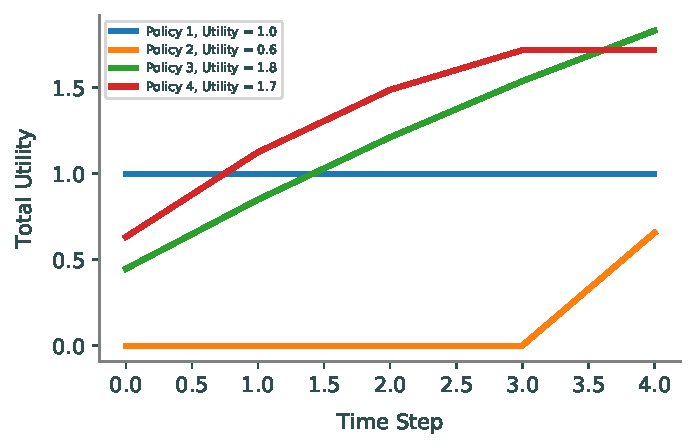
\includegraphics[width=.7\textwidth]{figures/diff_policies.pdf}
\caption{Plots for various policies with $u(x) = \sqrt{x}$ and $\beta = 0.9$.
Policy 1 eats all of the cake in the first step while policy 2 eats all of the cake in the last step.
Their difference in utility demonstrate the effect of the discount factor on waiting to eat.
Policy 3 eats the same amount of cake at each step, while policy 4 begins by eating $.4$ of the cake, then $.3$, $.2$, and $.1$.}
\label{fig:diff_pols}
\end{figure}


%The figure above graphs the total utility for the following four policy vectors with $u(x) = \sqrt{x}$ and $\beta = 0.9$..
%\begin{align*}
%Policy 1 =& [1, 0, 0, 0, 0]\\
%Policy 2 =& [0, 0, 0, 0, 1]\\
%Policy 3 =& [0.2, 0.2, 0.2, 0.2, 0.2]\\
%Policy 4 =& [.4, .3, .2, .1, 0]
%\end{align*}

%\begin{problem}
%
%Write a function called \li{graph_policy()} that accepts a policy vector $\mathbf{c}$, a utility function $u(x)$, and a discount factor $\beta$.
%Return the total utility gained with the policy input.
%Also display a plot of the total cumulative utility gained over time.
%Ensure that the policy that the user passes in sums to 1.
%Otherwise, raise a \li{ValueError}.
%Test your answer with $u(x) = \sqrt{x}$, $\beta = 0.9$, and the policy vectors used in Figure \ref{fig:diff_pols}.
%
%\end{problem}



\section*{The Value Function}

The cake eating problem is an optimization problem where we maximize utility.

\begin{align}\label{eq:dynamicopt-do6}
\max_{c_t}  &\sum_{t=0}^T \beta^t u(c_t) \\
\mbox{subject to } &\sum_{t=0}^T c_t = W \nonumber\\
&c_t \geq 0.\nonumber
\end{align}

One way to solve it is with the value function.
The value function $V(a,b,W)$ gives the utility gained from following an optimal policy from time $a$ to time $b$.

\begin{align*}
V(a,b,W) = \max_{c_t} & \sum_{t=a}^b \beta^tu(c_t) \\
\mbox{subject to } & \sum_{t=a}^b c_t = W \\
& c_t \geq 0.
\end{align*}
$V(0,T,W)$ gives how much utility we gain in $T$ days and is the same as Equation \ref{eq:dynamicopt-do6}.
$V(a, b, \frac{W}{2})$ gives how much utility we will gain by proceeding optimally from $t=a$ if half of a cake of size $W$ was eaten before time $t=a$.

Let $W_t$ represent the total amount of cake left at time $t$.
Observe that $W_{t+1} \leq W_t$ for all $t$, because our problem does not allow for the creation of more cake.
Notice that $V(t+1, T, W_{t+1})$ can be represented by $\beta V(t, T-1, W_{t+1})$, which is the value of eating $W_{t+1}$ cake later.
Then we can express the value function as the sum of the utility of eating $W_t-W_{t+1}$ cake now and $W_{t+1}$ cake later.

\begin{equation}\label{eq:dynamicopt-do1}
V(t, T, W_{t}) = \max_{W_{t+1}} \left(u(W_{t} - W_{t+1}) + \beta V(t, T-1, W_{t+1})\right)
\end{equation}
where $u(W_t - W_{t+1})$ is the value gained from eating $W_t - W_{t+1}$ cake at time $t$.

Let $\w = \begin{bmatrix}0 & \frac{1}{N} & \cdots & \frac{N-1}{N} & 1\end{bmatrix}\trp$.
We define the \emph{consumption matrix} $C$ by $C_{ij} = u(w_i - w_j)$.
Note that $C$ is an $(N+1) \times (N+1)$ lower triangular matrix since we assume $j\leq i$; we can't consume more cake than we have.
The consumption matrix will help solve the value function by calculating all possible value of $u(W_{t} - W_{t+1})$ at once.
At each time $t$, $W_t$ can only have $N+1$ values, which will be represented as $w_i = \frac{i}{N}$, which is $i$ pieces of cake remaining.
For example, if $N=4$, then $w=[0, .25, .5, .75, 1]\trp$, and $w_3 = 0.75$ represents having three pieces of cake left.
In this case, we get the following consumption matrix.
Notice that $C_{20} = u(w_2-w_0) = u(.5-0)$ and $C_{52} = u(w_5-w_2) = u(1-.25) = u(.75)$.

\[
\begin{bmatrix}
0 & 0 & 0 & 0 & 0 \\
u(0.25) & 0 & 0 & 0 & 0 \\
u(0.5) & u(0.25) & 0 & 0 & 0 \\
u(0.75) & u(0.5) & u(0.25) & 0 & 0 \\
u(1) & u(0.75) & u(0.5) & u(0.25) & 0 \\
\end{bmatrix}.
\]

\begin{problem}

Write a function that accepts the number of equal sized pieces that divides the cake $N$ and a utility function $u(x)$.
Assume $W=1$, and create a partition vector whose entries correspond to possible amounts of cake.
Return the consumption matrix.

\end{problem}


\subsection*{Solving the Optimization Problem}

As mentioned above, $V(t, T-1, W_{t+1})$ in \ref{eq:dynamicopt-do1} is a new value function problem with $a = t, b = T-1$, and $W = W_{t+1}$, making \ref{eq:dynamicopt-do1} a recursion formula.
By using the optimal value of the value function in the future, $V(t, T-1, W_{t+1})$, we can determine the optimal value for the present, $V(t, T, W_{t})$.
$V(t, T, W_{t})$ can be solved by trying each possible $W_{t+1}$ and choosing the one that gives the highest utility.


The $(N+1) \times (T+1)$ matrix $A$ that solves the value function is called the \emph{value function matrix}.
$A_{ij}$ is the value of having $w_i$ cake at time $j$.
$A_{0j}$ = 0 because there is never any value in having $w_0$ cake, $u(w_0) = u(0) = 0$.

Initially we do not know how much cake to eat at $t = 0$: should we eat one piece of cake ($w_1$), or perhaps all of the cake ($w_N$)?
It may not be obvious which option is best and that option may change depending on the discount factor $\beta$.

Instead of asking how much cake to eat at some time $t$, we ask how valuable $w_i$ cake is at time $t$.
We start at the last time period.
Since there is no value in having any cake left over when time runs out, the decision at time $T$ is obvious: eat the rest of the cake.
The amount of utility gained from having $w_i$ cake at time $T$ is given by $u(w_i)$.
So $A_{iT} = u(w_i)$.
Written in the form of (\ref{eq:dynamicopt-do1}),

\begin{equation}\label{eq:dynamicopt-do2}
A_{iT} = V(0, 0, w_{i}) = \max_{w_{j}} \left(u(w_{i} - w_{j}) + \beta V(0, -1, w_{j})\right) = u(w_{i}).
\end{equation}

This happens because $V(0,-1,w_j) = 0$.
As mentioned, there is no value in saving cake so this equation is maximized when $w_j = 0$.
All possible values of $w_{i}$ are calculated so that the value of having $w_i$ cake at time $T$ is known.

\begin{warn}
Given a time interval from $t=0$ to $t=T$ the utility of waiting until time T to eat $w_i$ cake is actually $\beta^Tu(W_{i})$.
However, through backwards induction, the problem is solved backwards by beginning with $t=T$ as an isolated state and calculating its value.
This is why the value function above is $V(0, 0, W_i)$ and not $V(T, T, W_i)$.
\end{warn}

For example, the following matrix results with $T=3$, $N=4$, and $\beta=0.9$.
\[
\begin{bmatrix}
0 & 0 & 0 & u(0) \\
0 & 0 & 0 & u(0.25) \\
0 & 0 & 0 & u(0.5) \\
0 & 0 & 0 & u(0.75) \\
0 & 0 & 0 & u(1) \\
\end{bmatrix}.
\]


\begin{problem}
Write a function that accepts a stopping time $T$, a number of equal sized pieces that divides the cake $N$, a discount factor $\beta$, and a utility function $u(x)$.
Return the value function matrix for $t=T$ (the matrix should have zeros everywhere except the last column).
Return a matrix of zeros for the policy matrix.
\label{prob:dynamicopt-eat-cake}
\end{problem}

Next, we use the fact that $A_{jT} = V(0,0,w_j)$ to evaluate the $T-1$ column of the value function matrix, $A_{i(T-1)}$, by modifying  (\ref{eq:dynamicopt-do2}) as follows,
\begin{equation}\label{eq:dynamicopt-do3}
A_{i(T-1)}( = V(0, 1, w_{i}) = \max_{w_j}\left(u(w_{i} - w_{j}) + \beta V(0,0,w_{j})\right) = \max_{w_j}\left(u(w_{i} - w_{j}) + \beta A_{jT})\right).
\end{equation}

Remember that there is a limited set of possibilities for $w_j$, and we only need to consider options such that $w_j \leq w_i$.
Instead of doing these one by one for each $w_i$, we can compute the options for each $w_i$ simultaneously by creating a matrix.
This information is stored in an $(N+1) \times (N+1)$ matrix known as the \emph{current value matrix}, or $CV^t$, where the $(ij)$th entry is the value of eating $w_i-w_j$ pieces of cake at time $t$ and saving $j$ pieces of cake until the next period.
For $t = T-1$,
\begin{equation}\label{eq:dynamicopt-do4}
CV^{T-1}_{ij} = u(w_i - w_j) + \beta A_{jT}.
\end{equation}

The largest entry in the $i$th row of $CV^{T-1}$ is the optimal value that the value function can attain at $T-1$, given that we start with $w_i$ cake.
The maximal values of each row of $CV^{T-1}$ become the column of the value function matrix, $A$, at time $T-1$.
We then compute $CV^{T-2}$ using $A_{j(T-1)}$ and iterate backwards to fill in the rest of $A$.

\begin{warn}
The notation $CV^t$ does not mean raising the matrix to the $t$th power; rather, it indicates what time period we are in.
All of the $CV^t$ could be grouped together into a three-dimensional matrix, $CV$, that has dimensions $(N+1) \times (N+1) \times (T+1)$.
Although this is possible, we will not use $CV$ in this lab, and will instead only consider $CV^t$ for any given time $t$.
\end{warn}

The following matrix is $CV^{2}$ where $T=3$, $\beta = .9$, $N=4$, and $u(x) = \sqrt{x}$.
The maximum value of each row, circled in red, is used in the $3^{rd}$ column of $A$.
Remember that $A$'s column index begins at $0$, so the $3^{rd}$ column represents $j=2$.

\begin{center}
\begin{tikzpicture}
%Style for making the nodes with ellipse border
\tikzstyle{ell}=[ellipse,draw=red,fill=none,
text centered,minimum height=.5em,text width=.5cm]
\tikzstyle{ell2}=[ellipse,draw=red,fill=none,
text centered,minimum height=.5em,text width=.7cm]
\node at (-4,0) {$CV^2=$};
%Create the matrix with the ell nodes
\matrix[matrix of math nodes,left delimiter={[},right delimiter={]}]{
    \node[ell] {0}; & 0 & 0 & 0 & 0 & \\
    \node[ell] {0.5}; & 0.45 & 0 & 0 & 0 & \\
    0.707 & \node[ell] {0.95}; & 0.636 & 0 & 0 & \\
    0.866 & \node[ell2] {1.157}; & 1.136 & 0.779 & 0 & \\
    1 & 1.316 & \node[ell2] {1.343}; & 1.279 & 0.9 & \\
};
\end{tikzpicture}
\end{center}

Now that the column of A corresponding to $t = T-1$ has been calculated, we repeat the process for $T-2$ and so on until we have calculated each column of A.
In summary, at each time step $t$, find $CV^t$ and then set $A_{it}$ as the maximum value of the $i$th row of $CV^t$.
Generalizing \eqref{eq:dynamicopt-do3} and \eqref{eq:dynamicopt-do4} shows
\begin{equation}\label{eq:dynamicopt-do5}
CV^{t}_{ij} = u(w_i - w_j) + \beta A_{j(t+1)}.
\qquad \qquad
A_{it} = \max_{j} \left(CV_{ij}^t \right).
\end{equation}

The full value function matrix corresponding to the example is below.

\begin{figure}[H]
\[
A =
\begin{bmatrix}
0 & 0 & 0 & 0 \\
0.5 & 0.5 & 0.5 & 0.5 \\
0.95 & 0.95 & 0.95 & 0.707 \\
1.355 & 1.355 & 1.157 & 0.866 \\
1.7195 & 1.562 & 1.343 & 1 \\
\end{bmatrix}
.
\]
\caption{The value function matrix where $T=3$, $\beta=.9$, $N=4$, and $u(x) = \sqrt{x}$. The bottom left entry indicates the highest utility that can be achieved is $1.7195$.}
\label{fig:2nd_val_func_matrix}
\end{figure}

\begin{problem}
Complete your function from Problem \ref{prob:dynamicopt-eat-cake} so it returns the entire value function matrix.
Starting from the next to last column, iterate backwards by
\begin{itemize}
\item calculating the current value matrix for time $t$ using (\ref{eq:dynamicopt-do5}),
\item finding the largest value in each row of the current value matrix, and
\item filling in the corresponding column of $A$ with these values.
\end{itemize}
\end{problem}

\subsection*{Solving for the Optimal Policy} % --------------------------------

With the value function matrix constructed, the optimization problem is solved in some sense.
The value function matrix contains the maximum possible utility to be gained.
However, it is not immediately apparent what policy should be followed by only inspecting the value function matrix $A$.
The $(N+1) \times (T+1)$ policy matrix, P, is used to find the optimal policy.
%The calculation of $A$ involves the policy - we just didn't keep track of it. %Sounds too casual.
The $(ij)$th entry of the policy matrix indicates how much cake to eat at time $j$ if we have $i$ pieces of cake.
Like $A$ and $CV$, $i$ and $j$ begin at $0$.

The last column of P is calculated similarly to last column of A.
$P_{iT} = w_i$, because at time $T$ we know that the remainder of the cake should be eaten.
Recall that the column of $A$ corresponding to $t$ was calculated by the maximum values of $CV^{t}$.
The column of $P$ for time $t$ is calculated by taking $w_i - w_j$, where $j$ is the smallest index corresponding to the maximum value of $CV^{t}$,
\[
P_{it} = w_i - w_j.
\]
\begin{align*}
\mbox{where} \, \, & j = \{\, min\{j\} \mid CV_{ij}^t \geq CV_{ik}^t \, \forall \, k \in \left[0,1, \ldots , N \right] \,\}
\end{align*}

Recall $CV^2$ in our example with $T=3$, $\beta=.9$, $N=4$, and $u(x) = \sqrt{x}$ above.

\begin{center}
\begin{tikzpicture}
%Style for making the nodes with ellipse border
\tikzstyle{ell}=[ellipse,draw=red,fill=none,
text centered,minimum height=.5em,text width=.5cm]
\tikzstyle{ell2}=[ellipse,draw=red,fill=none,
text centered,minimum height=.5em,text width=.7cm]
\node at (-4,0) {$CV^2=$};
%Create the matrix with the ell nodes
\matrix[matrix of math nodes,left delimiter={[},right delimiter={]}]{
    \node[ell] {0}; & 0 & 0 & 0 & 0 & \\
    \node[ell] {0.5}; & 0.45 & 0 & 0 & 0 & \\
    0.707 & \node[ell] {0.95}; & 0.636 & 0 & 0 & \\
    0.866 & \node[ell2] {1.157}; & 1.136 & 0.779 & 0 & \\
    1 & 1.316 & \node[ell2] {1.343}; & 1.279 & 0.9 & \\
};
\end{tikzpicture}
\end{center}

To calculate $P_{12}$, we look at the second row ($i=1$) in $CV^2$.
The maximum, $.5$, occurs at $CV_{10}^2$, so $j=0$ and $P_{12} = w_1-w_0 = .25-0$.
Similarly, $P_{42} = w_4-w_2 = 1-.5 = .5$.
Observe that the $j$th index corresponds to the red ovals.
Continuing in this manner,
\begin{center}
\begin{tikzpicture}
%Style for making the nodes with ellipse border
\tikzstyle{ell}=[ellipse,draw=red,fill=none,
text centered,minimum height=.5em,text width=.5cm]
%Create the matrix with the ell nodes
\node at (-3,0) {$P=$};
\matrix[matrix of math nodes,left delimiter={\lbrack},right delimiter={\rbrack}]{
    0    & 0    & 0    & 0    & \\
    0.25 & 0.25 & 0.25 & \node[ell] (4) {0.25}; & \\
    0.25 & 0.25 & \node[ell] (3) {0.25}; & \node[ell,draw=blue] (6) {0.5};  & \\
    0.25 & \node[ell] (2) {0.25}; & 0.5  & 0.75 & \\
    \node[ell] (1) {0.25}; & 0.5  & \node[ell,draw=blue] (5) {0.5};  & 1.   & \\
};
%Arrows
\foreach \s/\t in {1/2,2/3,3/4}
{\draw[->,>=stealth',red](\s)--(\t);}
\draw[->,>=stealth',blue](5)--(6);
\end{tikzpicture}
\end{center}

The optimal policy is found by starting at the $(ij)$th entry where $i$ is the number of slices of cake available at the $j$th time interval.
At each time intervals, eat as much cake as the $(ij)$th entry indicates, as traced out by the red arrows.
So when $N=4$ and $j=0$, we eat $A_{40}=.25$ cake.
Then at the next time interval, $j=1$, $N=3$ so we eat $A_{31}=.25$ of the cake.
The blue arrows trace out the policy that would occur if we only had $2$ time intervals instead of $4$.
In this case, we need to start at $j=2$ so that the last time interval $T=3$ corresponds to the second time interval, when $j=3$.
What would be the optimal policy if we had $3$ time intervals?


\begin{center}
\begin{tikzpicture}

%Create the matrix with the ell nodes
\matrix[matrix of math nodes,left delimiter={\lbrack},right delimiter={\rbrack},font=\tiny]{
0 & 0 & 0 & 0 \\
\sqrt{0.25} & \sqrt{0.25} & \sqrt{0.25} & \sqrt{0.25} \\
\sqrt{0.25} + \beta\sqrt{0.25} & \sqrt{0.25} + \beta\sqrt{0.25} & \sqrt{0.25} + \beta\sqrt{0.25} & \sqrt{0.5} \\
\sqrt{0.25} + \beta\sqrt{0.25} + \beta^2\sqrt{0.25} & \sqrt{0.25} + \beta\sqrt{0.25} + \beta^2\sqrt{0.25} & \sqrt{0.5} + \beta\sqrt{0.25} & \sqrt{0.75} \\
\sqrt{0.25} + \beta\sqrt{0.25} + \beta^2\sqrt{0.25} + \beta^3\sqrt{0.25} & \sqrt{0.5} + \beta\sqrt{0.25} + \beta^2\sqrt{0.25} & \sqrt{0.5} + \beta\sqrt{0.5} & \sqrt{1} \\
};
%Matrix name and colored lines
\node at (-6,0) {$A=$};
\draw[red,very thick] (-5,-1.025) -- (-.9,-1.025);
\draw[blue,very thick] (2.6,-1.025) -- (4.1,-1.025);
\end{tikzpicture}
\end{center}

The non-simplified version of Figure \ref{fig:2nd_val_func_matrix}. Notice that the value of $A_{ij}$ is equal to following optimal path if you start at $P_{ij}$.
$A_{40}$ has the same values traced by the red arrows in $P$ above and $A_{42}$ has the same values traced by the blue arrows.

\begin{problem}
Modify your function from Problem \ref{prob:dynamicopt-eat-cake} to determine the policy matrix.
Initialize the matrix as zeros and fill it in starting from the last column at the same time that you calculate the value function matrix.
\\(Hint: You may find \li{np.argmax()} useful.)
\end{problem}

\begin{problem}
The $(ij)$th entry of the policy matrix tells us how much cake to eat at time $j$ if we start with $i$ pieces.
Use this information to write a function \li{find_policy()} that will find the optimal policy for the stopping time $T$, a cake of size 1 split into $N$ pieces, a discount factor $\beta$, and the utility function $u$.

%Replacing problem 1: graph_policy
%Use \li{graph\_policy()} to plot the optimal policy.
%See Figure \ref{fig:optimal_policy_graph} for an example.

%TODO: Figure out how to put graph in plots.py
%\begin{figure}[H]
%\includegraphics[width=.7\textwidth]{figures/optimal_policy_graph.pdf}
%\caption{The graph of the optimal policy (Policy 3 from Figure \ref{fig:diff_pols}) where $T=4$, $\beta=.9$, $N=5$, and $u(x) = \sqrt{x}$. It achieves a value of roughly $1.83$.}
%\label{fig:optimal_policy_graph}
%\end{figure}

\end{problem}







\begin{comment}
%
% This is the old version of the lab.  I am keeping it in for now.
% If we wish to expand this lab then this material may help write
% more sections, i.e. infinite horizon problems.
%

\section*{The Sequential Problem, Finite Horizon}
Suppose there are time periods $t=0,1,\ldots, T$ and at each time period we take an action $c_t$. Furthermore, at the beginning
of each time period $t$ we are in some state $W_t$.  In many cases $W_t$ might represent an available resource, such as money.
At each time we receive some reward, $u(W_t,c_t)$, for taking action $c_t$ given state $W_t$.  We assume that rewards are worth
more now than later. We let $\beta\in (0,1)$ represent what is called the discount factor, which gives the ratio of preference for
rewards today versus rewards tomorrow.  For example, receiving a dollar today is preferable to receiving a dollar in a year
because taking a dollar today and putting it into a savings account results in having more than a dollar in a year.  Lastly, over
time our state variable $W_t$ changes according to some rule depending on the previous state and our actions,
\begin{equation}
\label{motion}
W_{t+1} = g(W_t,c_t).
\end{equation}
Equation \eqref{motion} is sometimes referred to as the law of motion, as it describes how we move from state to state.
Mathematically such a problem can be represented as follows:
\begin{equation*}
\text{maximize} \sum_{t=0}^T \beta^t u(W_t,c_t) \quad \text{s.t.} \quad W_{t+1} = g(W_t,c_t)
\end{equation*}
where our initial state, $W_0$, is given.  There may also be restrictions on our choices $c_t$.  For example, in many applications
the state $W_t$ represents the amount of some resource available, and $c_t$ represents the amount we use up in time period $t$.
 In this case we would require $c_t \in [0,W_t]$.

For simplicity, lets assume that $u$ is a function of $c_t$ only (this is often, though not always, the case in practice).
 First let's consider the case that $T=0$.  So we maximize
\begin{equation}\label{1perprob}
u(c_0)
\end{equation}
over $c_0 \in [0,W_0]$.  In most cases $u$ is increasing, which we will assume here.  In this case it will be optimal to choose
 the largest value of $c_0$ possible, that is, $c_0 = W_0$.  Thinking of $W_0$ as our available resources, this simply means
 that if we don't have future periods to consider, we will use all of it.

In fact, this is always true in the last period.  In a problem with $T$ periods we know that we will use all of our resources
remaining in period $T$.  Consider the two period problem:
\begin{equation}
\label{2perprob}
\max \, \{u(c_0) + \beta u(c_1)\}
\end{equation}
where $c_0 \in [0,W_0]$, $c_1 \in [0,W_1]$ and $W_1 = g(W_0,c_0)$.  We know that in the last period we will use all of our
remaining resources, so $c_1 = W_1=g(W_0,c_0)$.  Substituting gives
\begin{equation}
\label{2perproba}
\max \, \{u(c_0) + \beta u(g(W_0,c_0))\}.
\end{equation}
Now we need only determine $c_0$.  Taking the derivative of \eqref{2perproba} with respect to $c_0$ and setting equal to zero
gives the first order condition
\begin{equation}
\label{FOC}
u'(c_0) = -\beta u'(g(W_0,c_0))g_c(W_0,c_0)
\end{equation}
where $g_c$ is the partial derivative of $g$ with respect to $c_0$.

Given a specific form for $u$ we could solve for $W_1$ and obtain the optimal solution.  In fact, we can solve a problem of
any length $T$ in this manner, by starting at the last time period and working backward.  We know that $W_{T+1} = 0$.  Working
backward in time we obtain an equation at each time step $t<T$ by taking the derivative with respect to $c_t$ and setting the equation equal to zero.  This process is called backward induction.  The equations at each time step, such as equation \eqref{FOC}, are sometimes called the inter-temporal Euler equations.  These equations, along with $c_T = W_T$, make $T+1$ equations to go with our $T+1$ unknowns $\{c_0,c_1,c_2,\ldots,c_T\}$, where we can use the law of motion \eqref{motion} to relate the $c_t$ and $W_t$

\section*{The Recursive Problem, Finite Horizon}
Approaching the problem sequentially like this can be somewhat messy.  The dynamic programming approach we consider now is more
easily adaptable to many situations.  The key to the dynamic programming approach is to define the optimization problem in terms
 of subproblems.  Notice that if we are in time period $t$, we face a problem of exactly the same form as the problem at time
 $0$.  We are in some state $W_t$, and want to maximize the sum from $t$ to $T$.  With this idea in mind, we define a function
  $V_t(W_t)$ called the value function.  The function $V_t$ gives the value of entering time $t$ in state $W_t$ and making
  optimal decisions moving forward.  So
\begin{equation*}
V_{t-1}(W_{t-1}) = \max_{c_t} \left\{u(c_{t-1}) + \beta V_t(g(W_{t-1},c_{t-1}))\right\}.
\end{equation*}
This is called the Bellman Equation.  The key to this formulation is that we decide what to do in period $t-1$ with the
assumption that our actions in the remaining periods will be optimal.  This is called the principal of optimality.

Let us consider a specific example from economics called The Cake Eating Problem.  Suppose $W_t$ represents the amount of
cake available at time $t$.  At each time period we can choose how much to consume.  What we eat, $c_t$, gives us a reward.
What we save, $W_t-c_t$, does not give us a reward (until it is eaten in a later period).  The law of motion \eqref{motion}
becomes
\begin{equation}\label{LOM_EX}
W_{t+1} = g(W_t,c_t) = W_t-c_t
\end{equation}

Now we have completely defined the problem.  The Bellman Equation is
\begin{equation*}
V_{t-1}(W_{t-1}) = \max_{c_t} \left\{u(c_{t-1}) + \beta V_t(W_{t-1}-c_{t-1})\right\}.
\end{equation*}
Notice that by the law of motion, each $c_t$ is determined by $W_t$ and $W_{t+1}$.
In fact, rearranging \eqref{LOM_EX}, we have
\begin{equation*}
c_t = W_t - W_{t+1}.
\end{equation*}
We can therefore rewrite the value function as
\begin{equation}
V_{t-1}(W_{t-1}) = \max_{W_t} \left\{u(W_{t-1} - W_{t}) + \beta V_t(W_t)\right\}.
\label{cake_valfn}
\end{equation}

We see that determining the optimal actions $c_t$ is equivalent to determining the optimal states $W_{t}$ in the
above formulation. The solution to this
problem is often called a \emph{policy function}.  A policy function determines an action based on the current
state.  Denoting the policy function by $\psi$, this can be written as
\begin{equation*}
W_{t+1}=\psi_t \left(W_t\right).
\end{equation*}
The policy function gives the optimal amount of cake to leave for the next period (equivalent to the amount of consumption) given
the amount of cake at the start of the period.  In other words, it determines the choice of $W_t$ that satisfies the $\max$
condition in \eqref{cake_valfn}.

As before, we know that in the last time period we should not save anything.  So $V_{T+1}(W_{T+1}) = 0$, i.e. there is
no value in leaving wealth for period $T+1$. Stated in another way, our action at time $T$ should be to eat all of the
remaining cake $W_T$, so $W_{T+1} = \psi_T(W_T) = 0$.
Plugging this result into the Bellman Equation gives us $V_T(W_T) = u(W_T)$.
Now consider the value function equation for period $T-1$:
\begin{align*}
V_{T-1}(W_{T-1}) &= \max_{W_T} \left\{u(W_{T-1} - W_T) + \beta V_T(W_T)\right\} \\
                 &= \max_{W_T} \left\{u(W_{T-1} - W_T) + \beta u(W_T)\right\}.
\end{align*}
We can determine this value by optimizing over $W_T$, where $0 \leq W_T \leq W_{T-1}$.
Continuing backwards in this manner leads us to the solution of the original problem.

\begin{problem}
\label{prob:cake_prob}
We recommend reading the entire problem before beginning to work on it, as many questions may be addressed further on.  This applies to the other problems in this lab as well.

Follow the steps below to solve the problem described above.  Take $u(c_t) = \sqrt{c_t}$.
You will write a function called \li{eatCake} that takes parameters $\beta$ (the discount factor),
$N$ (the number of discrete cake values to consider), $W_{max}$ (the original size of the cake,
set to the default value of $1$), a keyword argument \li{finite} (set to default value \li{True}),
a keyword argument  $T$ (the number of time periods, set to
default value \li{None}), and a keyword argument \li{plot}, which indicates whether or not
to plot the computed results. The function should return arrays representing the value function and the
policy function (we describe how to compute these in the following steps).
\begin{enumerate}
\item Approximate the continuum of possible cake sizes by creating an array
of evenly-spaced values that range from to 0 to $W_{max}$ inclusive.
Let the number of possible cake values be given by $N$. In Python, this can be accomplished easily by
using the \li{linspace} function in NumPy. You should obtain an array (call it $w$) of the form
\[
w = (w_1, w_2, \ldots, w_N),
\]
where $w_1 = 0$ and $w_N = W_{max}$.

\item Note that in order to compute the value function, we need $u(W_{t-1}-W_t)$.
We will pre-compute all such possible values and store them in an array, as follows:
Create an $N$ by $N$ matrix that contains
all possible values of $W_{t-1} - W_t$ (where $W_{t-1}$ corresponds to rows and $W_{t}$ to columns).  Make sure that
$c_t \geq 0$ is satisfied by replacing negative entries in the matrix with zeros.  Then take the square root to get a matrix
of $u(W_{t-1}-W_t)$.  To make sure we do not choose $W_{t-1} - W_t < 0$ when maximizing, replace the corresponding entries of
the $u(W_{t-1}-W_t)$ matrix with a large negative number (e.g. $-10^{10}$). You should end up with a matrix whose
$(i,j)$-th entry is equal to $\sqrt{w_i - w_j}$ when $i \geq j$, and is equal to $-10^{10}$ when $i < j$.

\item Next, create an $N$ by $T+2$ (corresponding to $t=0,1,\ldots, T+1$) matrix representing the value function for a given
time $t$ and state $W_t$.  We can initialize it with zeros and begin filling in the columns starting with the last (which we
know is zeros), as explained below.

\item Now we are ready to iterate backward and compute the value function for each time period.  To find $V_T$, we first compute
$u(W_T - W_{T+1}) + \beta V_{T+1}(W_{T+1})$ for all values of $W_{T}$ and $W_{T+1}$.  This will result in an $N$ by $N$ matrix
where the rows correspond to values of $W_{T}$ and the columns correspond to values of $W_{T+1}$.
%Note that to compute this
%we need a matrix representing $\beta V_{T+1}(W_{T+1})$.  Because this quantity does not depend on $W_T$, its rows should be
%equal.  To do this, we want to take $\beta V_{T+1}(W_{T+1})$ as a row vector and stack this vector to create a matrix with
%equal rows.  There are multiple ways to do this.  One is the \li{np.repeat} function.  For example, if \li{b} is a row vector
%it could be used like the following.
%\begin{lstlisting}
%b = [[1, 2, 3]]
%np.repeat(b, 3, axis = 0)
%array([[1, 2, 3],
%[1, 2, 3],
%[1, 2, 3]])
%\end{lstlisting}
%In general, be careful about having the correct rows, columns, transposes, etc throughout your code.

Now we maximize over choices of $W_{T+1}$ (choosing how much to save for the next period).  Then we will have a row vector
representing the value function for period $T$ across all possible $W_{T+1}$.  Iterate this procedure to fill in the value
function for all $t=T+1,T,\ldots, 0$.

\item In each iteration, you maximize to find the value function at time $t$.  Save the values of $W_{t+1}$ that achieve the
maximum.  The result is an $N$ by $T+1$ matrix whose $(n,t)$ entry gives the optimal amount of cake to leave for period
$t+1$, given that we start period $t$ with the $n$-th value of our vector of cake.  This is the policy function.

\item If the keyword argument \li{plot} is set to \li{True}, plot the surface of the Value and Policy functions.
This can be done by including the following import lines
\begin{lstlisting}
>>> from matplotlib import pyplot as plt
>>> from matplotlib import cm
>>> from mpl_toolkits.mplot3d import Axes3D
\end{lstlisting}
and using the following code:
\begin{lstlisting}
>>> W = np.linspace(0, Wmax, N)
>>> x = np.arange(0, N)
>>> y = np.arange(0, T+2)
>>> X, Y = np.meshgrid(x, y)
>>> fig1 = plt.figure()
>>> ax1 = Axes3D(fig1)
>>> ax1.plot_surface(W[X], Y, np.transpose(V), cmap=cm.coolwarm)
>>> plt.show()

>>> fig2 = plt.figure()
>>> ax2 = Axes3D(fig2)
>>> y = np.arange(0,T+1)
>>> X, Y = np.meshgrid(x, y)
>>> ax2.plot_surface(W[X], Y, np.transpose(psi), cmap=cm.coolwarm)
>>> plt.show()
\end{lstlisting}
where \li{W} is the vector of cake amounts, \li{V} is the value function, and \li{psi} is the policy function.

\item Return the arrays giving the value function and the policy function.
\end{enumerate}

Solve the problem using cake size $1$, discount factor $\beta = .9$, number of time periods $T = 10$, and number of
discrete cake values $N = 100$. You should also try plotting the value and policy functions for fixed time periods across
$W_t$, or for fixed $W_t$ across time,
 and make sure that these plots fit your intuition. See Figure \ref{fig:valueslices}. Your output should
agree with the figure.
\end{problem}

\begin{figure}
\begin{subfigure}{.5\textwidth}
    \includegraphics[width=\textwidth]{figures/fixed_time.pdf}
\end{subfigure}
\begin{subfigure}{.5\textwidth}
    \includegraphics[width=\textwidth]{figures/fixed_w.pdf}
\end{subfigure}
\caption{Slices of the finite horizon value function for fixed values of $t$ and $W$, respectively.}
\label{fig:valueslices}
\end{figure}

\section*{The Recursive Problem, Infinite Horizon}\label{SecRecProbInFHor}
Next we consider an infinite horizon problem.  For simplicity, we continue with the example from the previous section.
Suppose that rather than optimizing over $t = 0,1,\ldots,T$, we wish to optimize over an infinite time horizon:
\begin{equation*}
\text{maximize} \sum_{t=0}^\infty \beta^t u(W_t,c_t) \quad \text{s.t.} \quad W_{t+1} = g(W_t,c_t).
\end{equation*}
Since at any time $t$, there are an infinite number of periods remaining, one might suspect that the optimal policy will
not depend on the current time $t$.

\begin{problem}
\label{prob:cake_prob2}
Compute the solution to Problem \ref{prob:cake_prob} with $T = 1000$, and the rest of the inputs the same.
Plot the policy function across time for fixed $W_t = 1$.
Notice that it is the same for all time periods, except those near the end time $T$.
\end{problem}

As suggested by the results of Problem \ref{prob:cake_prob2},  the policy function for the infinite horizon problem does not
depend on the time $t$ (this can be proved).  That is, at any time $t$, the optimal decision depends only on the amount of cake
at the beginning of the period, not the value of $t$.  So everything can now be written in terms of variables today and variables
tomorrow. We will denote variables tomorrow with a ``$\:'\:$".
\begin{equation}
\label{EqBellman}
V\left(W\right) = \max_{W'\in[0,W]}\:\: \left\{u\left(W - W'\right) + \beta V\left(W'\right)\right\}
\end{equation}
Note that the value function $V$ on the left-hand-side of \eqref{EqBellman} and on the right-hand-side are the same function.

Because the problem now has an infinite horizon, the nature of the solution is a little different. The solution to \eqref{EqBellman}
is a policy function $W'=\psi(W)$ that creates a fixed point in $V$. In other words, the solution is a policy function $\psi(W)$
that makes the function $V$ on the left-hand-side of \eqref{EqBellman} equal the function $V$ on the right-hand-side.

Define $C$ as an operator on any value function $V_k\left(W\right)$. Let $C$ perform the following operation.
\begin{equation}
\label{EqContraction}
C\Bigl(V_k\left(W\right)\Bigr) \equiv \max_{W'\in[0,W]}\:\: \left\{u\left(W-W'\right) + \beta V_k\left(W'\right)\right\}.
\end{equation}
Note that the value function on the right-hand-side of \eqref{EqContraction} and on the left-hand-side are the same function $V_k$,
but have different inputs--$W$ versus $W'$. The operator $C$ takes in a function $V_k$, and gives a new
function which we will call $V_{k+1}$:
\begin{equation*}
V_{k+1}\left(W\right) \equiv C\Bigl(V_k\left(W\right)\Bigr).
\end{equation*}
The value function $V_{k+1}$ that results from the operation $C$ is not necessarily the same as the value function that the system
began with ($V_k$). However, according to equation \eqref{EqBellman} we seek a $V$ such that $C(V) = V$.  The solution, then, is the fixed point in $V$.
\begin{equation*}
C\Bigl(V_k\left(W\right)\Bigr) = V_{k+1}\left(W\right) = V_k\left(W\right) = V\left(W\right)
\end{equation*}

When trying to solve a fixed point equation, it is often very helpful to utilize the Contraction Mapping Principle, which
guarantees the existence of a fixed point of a mapping, provided that the map sends any two distinct inputs to outputs
that are strictly closer to each other than the inputs, in a controlled way. This principle also provides a constructive
way to obtain the fixed point, namely by iterating the map.
Fortunately, it can be shown that if $u(\cdot)$ is real-valued, continuous, and bounded, $\beta\in(0,1)$, and that the constraint
set $W'\in[0,W]$ is nonempty, compact-valued, and continuous, then the operator $C$ is a contraction and thus we can obtain
a solution $V$ by iteration:
\begin{equation*}
\lim_{k\rightarrow\infty}\: C^k\Bigl(V_0\left(W\right)\Bigr) = V_k(W) =  V\left(W\right)
\end{equation*}
for any $V_0$.

Remember, in the infinite horizon problem both the value and policy functions do not depend on time.  Computationally, this means that
 the value and policy functions in the infinite horizon problem are one dimensional.

\begin{problem}
Expand your \li{eatCake} function to solve the Cake Eating Problem with an infinite time horizon. If the keyword argument
\li{finite} has the value \li{True}, then your function should behave as in Problem \ref{prob:cake_prob}, solving the finite
time horizon problem. However, if \li{finite = False}, solve the infinite time horizon problem through the following steps.
Both problems will require you to pre-compute the values $u(W - W')$, where $W$ and $W'$ range over the set of discrete cake
amounts. Be sure to avoid replicating code by factoring it out.
As in Problem \ref{prob:cake_prob}, take $u(c_t) = \sqrt{c_t}$.
\begin{enumerate}
\item As in Problem \ref{prob:cake_prob}, approximate the continuum of possible
cake sizes by a column vector called $W$ that ranges from 0 to $W_{max}$ in $N$ steps.

\item \label{item:step2} Initialize the value function V as a vector of zeros of length $N$.  This is $V_0$.  Perform one iteration
of the contraction operation given in equation \eqref{EqContraction} to get a new value function $V_1$ (this should be very similar
to Problem 1).  Determine the resulting policy function $W' = \psi_1\left(W\right)$.  [HINT: The policy function should be a vector
of length $N$ of optimal future values of the cake $W'$ given the current value of the cake $W$, and $V_T$ should be an $N$-length
vector representing the value of entering a period with cake size $W$.]

\item \label{item:step3} Measure the distance between the two value functions as the sum of the
squared differences,
\begin{equation}
\label{EqDist}
\delta_1\equiv \norm{V_1\left(W\right) - V_0\left(W'\right)}_2^2 = \left(V_1 - V_0\right)^T\left(V_1 - V_0\right).
\end{equation}
Defined in this way, $\delta_1\in [0,\infty)$.

%\item \label{item:step4} Take the resulting $V_1$ from \ref{item:step2}, and perform the same contraction on it to generate $V_2$
%and $\psi_2$. That is, generate,
%\begin{equation*}
%  V_2\left(W\right) = C\Bigl(V_1\left(W\right)\Bigr) = \max_{W'\in[0,W]}\: u\left(W - W'\right) + \beta V_1\left(W'\right)
%\end{equation*}
%and the accompanying policy function $W'=\psi_2\left(W\right)$. Calculate the accompanying distance measure for $\delta_2$ using
% the formula from \eqref{EqDist} with the updated period subscripts. Compare $\delta_2$ with $\delta_1$ from \ref{item:step3}.
%
%\item \label{item:step5} Repeat \ref{item:step4} and generate $V_3$ and $\psi_2$ by performing the contraction on $V_2$. Compare
%$\delta_3$ to $\delta_2$ and $\delta_1$.

\item Write a loop that performs the contraction operation from steps \ref{item:step2} and \ref{item:step3} iteratively
until the distance measure is very small ($\delta_k < 10^{-9}$).  The distance measure $\delta_k$ being arbitrarily close to zero means
 you have converged to the fixed point $V_k = V_{k+1} = V$. (For fun, you can show that the policy function converges to the same
 function regardless of what you put in for your initial policy function value.)

\item If \li{plot = True}, plot the converged policy function vector
($y$-axis) as a function of the cake amounts ($x$-axis).

\item Return the value function and policy function arrays.

Compute the value function and policy function for the infinite time horizon problem with
cake size $1$, discount factor $\beta = .9$, and number of
discrete cake values $N = 100$. The plot you generate should agree with Figure \ref{fig:infinitePolicy}.
\end{enumerate}
\end{problem}

\begin{figure}
\includegraphics[width=\textwidth]{figures/infiniteHorizon.pdf}
\caption{Policy function for infinite time horizon.}
\label{fig:infinitePolicy}
\end{figure}

\begin{figure}
\includegraphics[width=\textwidth]{figures/convergence.pdf}
\caption{Due to the contraction mapping principle, $\delta_k$ decreases as we perform iterations
until it is small enough to meet our convergence tolerance.}
\end{figure}

\section*{Infinite Horizon, Stochastic, i.i.d.}\label{SecRecProbInfinHorStochiid}

In practice, dynamic programming problems often involve some level of uncertainty.
For example, as time progresses prices may fluctuate, resources may vary, or preferences themselves may change.
 In this lab, we reexamine the cake eating problem, this time allowing for uncertainty.

We consider again the problem of optimizing a sequence of decisions over an infinite time horizon.
We assume that the individual's preferences deviate each period according to some ``shock" $\ve$,
where $\ve$ is a random variable.  We assume that the shock terms $\ve$ for each time period are
independent and identically
distributed (i.i.d.).  In effect, this means the probabilities associated with the $\ve$ are the
same for any time $t$ and do not depend on each other.  We assume for now that the $\ve$ are
distributed normally with mean $\mu$ and variance $\sigma^2$.  The Bellman equation can be easily
rewritten in the following way to incorporate the uncertainty,
\begin{equation}\label{stoch_Bellman}
   V\left(W,\ve\right) = \max_{W'\in[0,W]}\: \{\ve u\left(W - W'\right) +
   \beta E_{\ve'}\left[V\left(W',\ve'\right)\right]\},
\end{equation}
where $\ve \sim N(\mu,\sigma^2)$ and
$E$ is the unconditional expectation operator over $\ve$.  Note that now the value function depends
on two variables.  It represents the value of entering the period with $W$, the amount of cake,
and a preference shock of $\ve$.  For example, in a period where the realization of $\ve$ is higher,
we will get more value from the cake eaten in the current period.  Because we do not know the value of
the shock in the next period $\ve'$, we consider only the expected value for future time.

As it turns out, we can solve this problem in a manner similar to the infinite horizon deterministic cake-eating
problem considered in the Value Function Iteration lab.  It is worth noting that in this case,
 the value and policy functions will be two dimensional, as they will depend on both $W$ and $\ve$.

In order to deal with $\ve$ computationally, we would like to represent it as a vector of possible values
it could take, along with the corresponding probabilities that it takes each of those values.  However,
$N(\mu,\sigma^2)$ is a continuous distribution, so we cannot represent every value $\ve$ could take.
We need a discrete distribution that approximates $N(\mu,\sigma^2)$.

To do this, we choose $N$ equally spaced points centered about the mean at which to approximate the
distribution. Call these values $\ve_1,\ldots,\ve_N$, and let the spacing between adjacent points be
given by $\delta$.
We can then break up the support of the distribution into $N$ bins, where adjacent bins share a common
endpoint. Call the endpoints of these bins $v_1,\ldots,v_{N+1}$. By choosing the endpoints to be
halfway between each $\ve_k$, we have the formula
\[
v_k = \ve_k - \frac{1}{2}\delta, \qquad k=1,\ldots,N
\]
and
\[
v_{N+1} = \ve_N + \frac{1}{2}\delta.
\]

\begin{figure}[h!]
\label{stoch1_fig1}
\begin{center}
\includegraphics[width = \textwidth]{figures/discnorm.pdf}
\end{center}
\caption{Discretization of $N(\mu,\sigma^2)$.  We approximate $P(\ve = \ve_k)$ by the area of the shaded region.}
\end{figure}

We can then associate $\ve_k$ with the area under the curve from $v_k$ to $v_{k+1}$.
In Python, we can find the area using the function \li{norm.cdf} found in the \li{stats} package.
The cdf (cumulative distribution function) gives the area under the curve from $-\infty$ to a specified value.
For example, in the following code, \li{eps} is the area under the curve from 0 to 1.

\begin{lstlisting}
>>> from scipy import stats as st
>>> mu = 0
>>> sigma = 1
>>> eps = st.norm.cdf(1,loc=mu,scale=sigma) - st.norm.cdf(0,loc=mu,scale=sigma)
\end{lstlisting}

In general, it is sufficient to take our points $\ve_k$ ranging from $\mu - 3\sigma$ to $\mu + 3\sigma$, as this
range contains about 99.7\% of the probability mass.

\begin{problem}
Write a function called \li{discretenorm} that accepts an integer $K$ representing the number of discrete points
desired, a mean $\mu$, and a standard deviation $\sigma$. It should return a length-$K$ vector of equally-spaced
values ranging from $\mu - 3\sigma$ to $\mu + 3\sigma$ inclusive,
and a length-$K$ vector containing the associated probabilities.
Plot the approximation of $N(0,1)$ using different values of $K$ to check that your results are plausible.
\end{problem}

Now that we have a discrete distribution for $\ve$, we can solve for the value and policy functions
determined by \eqref{stoch_Bellman}.

\begin{problem}
Complete the following steps to solve the problem described above.
Assume that the period utility function is $u(c)=\sqrt{c}$.
Write a function \li{stochEatCake}
that accepts parameters $\beta$ (discount factor), $N$ (number of discrete cake values),
a tuple of values \li{e_params}, $W_{max}$ (the original size of the cake, set to default value 1),
a keyword argument \li{iid} (set to default value \li{True}), and
a keyword argument \li{plot} (set to default value of \li{False}). Inside the function, carry out the steps
outlined below.

The argument \li{e_params} is a tuple consisting of the values needed to generate
the discrete approximation to $\ve$. In the present case, this tuple consists (in order) of
$K$ (the number of discrete approximations of $\ve$), $\mu$ (the
mean of the shock term $\ve$), and $\sigma$ (the standard deviation of the shock term $\ve$),
since these are the arguments we need to pass to our \li{discretenorm} function.

\begin{enumerate}
\item First, compute an approximation of $\ve$ using the \li{discretenorm} function created in Problem 1.
Use $K$ equally spaced points to approximate $N(\mu,\sigma^2)$. Denote the resulting $K$-length
vector of equally-spaced values by
\[e =(e_1,\ldots,e_K),
\]
and denote the $K$-length vector of the associated probabilities
by
\[\Gamma = (\Gamma_1,\ldots,\Gamma_K).
\]
Note that $\Gamma_k$ give the probability $P(\ve = e_k)$.

Since the values needed for the \li{discretenorm} function are contained in the \li{e_params} input,
we can feed these values directly into the function in the following way:
\begin{lstlisting}
>>> e, gamma = discretenorm(*e_params)
\end{lstlisting}
The \li{*} operator essentially unpacks the values of a tuple or list.

\item As done previously, create a vector
\[w = (w_1,\ldots,w_N)
\]
of possible cake sizes. This should be
a length-$N$ vector of equally spaced values from 0 to $W_{max}$, inclusive.

\item Represent the value function as a $N \times K$ matrix $v$, satisfying
\[
v_{i,j} = V(w_i, e_j).
\]
(The rows correspond to different values of $W$ and the columns correspond to different values of $\ve$.)
Initialize each entry of the matrix to 0.

Likewise, represent the policy function as a $N \times K$ matrix $p$, satisfying
\[
p_{i,j} = \psi(w_i,e_j).
\]
Initialize all entries to 0.

\item In order to evaluate the value function equation, we need to pre-compute $\ve u(W-W')$ for all values of
$\ve,W,W'$.
Begin by computing all possible values of $u(W-W')$, and storing these values in a $N \times N$ array,
as done before. Call this array $u$. Make sure that the upper triangular
entries of this array are equal to zero, as these entries correspond to consuming more cake than is
available, which is impossible.

The values $\ve u(W-W')$ will be represented by a three-dimensional array $\hat{u}$ of size
$N\times N\times K$, satisfying
\[
\hat{u}_{i,j,k} = v_{i,j}e_k.
\]
We can compute this array easily as follows:

\begin{lstlisting}
>>> import numpy as np
>>> u_hat = np.repeat(u, K).reshape((N,N,K))*e
\end{lstlisting}


\item We also need to compute $E_{\ve'}\Bigl[V\left(W',\ve'\right)\Bigr]$ for each value of $W'$.
The expected value is simply
\begin{equation*}
E_{\ve'}\Bigl[V\left(W',\ve'\right)\Bigr] = \sum_{k=1}^K \Gamma_kV(W',e_k').
\end{equation*}
The result is a length $N$ vector, call it $E$, satisfying
\[
E_i = E_{\ve'}\Bigl[V\left(w_i,\ve'\right)\Bigr] = \sum_{k=1}^K \Gamma_kv_{i,k}
\]
This calculation can be done by multiplying $\Gamma$ element-wise to each row of the
value function matrix $v$, and then summing along the rows. Something like the following
line of code should do the trick:
\begin{lstlisting}
>>> E = (v*gamma).sum(axis=1)
\end{lstlisting}

\item We can now compute the value function contraction
\begin{equation*}\label{EqContractStochiid}
C\Bigl(V\left(W,\ve\right)\Bigr) \equiv \max_{W'\in[0,W]}\:
\Bigl\{\ve u\left(W-W'\right) + \beta E_{\ve'}\Bigl[V\left(W',\ve'\right)\Bigr]\Bigr\}.
\end{equation*}
The first task is to create an $N \times N \times K$ array $c$ satisfying
\[
c_{i,j,k} = \hat{u}_{i,j,k} + \beta E_j.
\]
This can be done in any manner of ways. Below is a one-liner that does the job.
\begin{lstlisting}
>>> c = np.swapaxes(np.swapaxes(u_hat, 1, 2) + beta*E, 1, 2)
\end{lstlisting}

Now, for any $k$, for all $i < j$, set $c_{i,j,k}$ to a large negative number, say $-10^{10}$,
so that when maximizing over this array, we do not choose to consume more cake than is available.
Again, this can be done in a variety of different ways, but the following does the job concisely:
\begin{lstlisting}
>>> c[np.triu_indices(N, k=1)] = -1e10
\end{lstlisting}

Finally, maximize over the second axis of $c$ (which corresponds to different values of $W'$)
to obtain the updated value function matrix:
\begin{lstlisting}
>>> v_new = np.max(c, axis=1)
\end{lstlisting}
You can likewise update your policy function matrix as follows:
\begin{lstlisting}
>>> max_indices = np.argmax(c, axis=1)
>>> p = w[max_indices]
\end{lstlisting}

\item We now have our updated value function matrix $v_{new}$ as well as the
previous $v$, which we refer to here as $v_{old}$. As we iterate on the value function equation, we need a norm
\begin{equation*}
\delta = \|v_{new} - v_{old}\|_2
\end{equation*}
that measures the distance between these two value functions to determine convergence.
You may compute the norm using the SciPy function \li{scipy.linalg.norm}, or by direct calculation.
At the end of each iteration, make sure to set $v$ to $v_{new}$, so that the updates carry through the
loop.
Iterate on the contraction until $\delta < 10^{-9}$.

\item If \li{plot = True}, make a 3-D surface plot of the policy function for the converged problem
$W' = \psi\left(W,\ve\right)$ which gives the value of the cake tomorrow as a
function of the cake today  and the taste shock today.  Do the same for the value function.
Example code to create the value function plot is provided below.
\begin{lstlisting}
>>> x = np.arange(0,N)
>>> y = np.arange(0,K)
>>> X,Y = np.meshgrid(x,y)
>>> fig1 = plt.figure()
>>> ax1 = Axes3D(fig1)
>>> ax1.plot_surface(w[X], Y, v.T, cmap=cm.coolwarm)
>>> plt.show()
\end{lstlisting}
Creating the policy function plot is similar.

\item Return the converged value function matrix $v$ and policy function matrix $p$.


\end{enumerate}
Test your function using values $\beta = .9$, $N = 100$, $K = 7$, $\sigma = .5$, $\mu = 4\sigma$,
and \li{plot = True}.
The proper way to set this up and call the function is as follows:
\begin{lstlisting}
>>> e_params = (7, 4*.5, .5)
>>> stuff = stochEatCake(.9, 100, e_params, plot=True)
\end{lstlisting}
\end{problem}

\begin{figure}
    \centering
    \includegraphics[width = \textwidth]{figures/stoch_value.pdf}
    \caption{3D surface representing the value function for the Stochastic Cake-Eating problem.}
\end{figure}

\section*{Infinite Horizon, Stochastic, AR(1)}\label{SecRecProbInfinHorStochAR1}

In the previous example, we assumed that the shocks at time $t$ were independent of what happened in
previous periods.  Often a shock may depend on recent events.  We will assume now that the shocks are persistent,
meaning preferences in the current period are more likely to be close to what they were in the previous period.
We can characterize the persistence by what is called an autoregressive process of order one, denoted AR(1).
Such a process is defined as follows.
\begin{equation}\label{EqAR1shock}
\ve' = (1-\rho)\mu + \rho\ve + \nu' \quad\text{where}\quad \rho\in(0,1) \quad\text{and}\quad \nu\sim N(0,\sigma^2).
\end{equation}

Essentially, instead of allowing the shocks to have a mean which is independent of the past, the mean is now a
weighted average (weighted by $\rho$) of some $\mu$ and the previous realization of the shock, $\ve$.  As it turns
 out, we can approximate this process by thinking of it as a Markov Chain. This means we need to determine a
 discrete set of points representing possible values of $\ve$ and a Markov transition matrix that gives the
 probabilities of moving from one value of $\ve$ to another.  There are methods for determining the discrete
 approximation of $\ve$ with a Markov transition matrix.  These methods are beyond the scope of this section,
 but you can use the file \li{tauchenhussey.py} to implement them in the next problem.

The Bellman equation becomes the following, in which the only change from the i.i.d. shock case is that the
expectations operator is now conditional on the current shock $\ve$:

\begin{equation*}
   V\left(W,\ve\right) = \max_{W'\in[0,W]}\: \{\ve u\left(W - W'\right) +
   \beta E_{\ve'|\ve}\left[V\left(W',\ve'\right)\right]\},
\end{equation*}
where $\ve'$ is distributed according to \eqref{EqAR1shock}.
Let $\Gamma_{i,j}=P\left(\ve_j'|\ve_i\right)$ where $\ve_j'$ is the value of the shock in
the next period and $\ve_i$ is the value of the shock in the current period.
In other words, $\Gamma$ is the Markov transition matrix.

The solution to this problem is of the same type as that in the i.i.d. case, since the only difference is
the probability distributions of the $\ve$.

\begin{problem}
Expand your \li{stochEatCake} function to handle the case of AR(1) shock terms. The function should
handle this case for the parameter value \li{iid = False}, and should handle the previous case of
normally distributed i.i.d. shock terms for the parameter value \li{iid = True}. You will need to
add a few ``if ... else" statements, as well as implement the steps outlined below, but most of the
code will remain unchanged.

\begin{enumerate}
\item In the AR(1) case, the \li{e_params} argument should be a tuple of values needed to
generate the arrays $e$ and $\Gamma$ that approximate the values and distribution of $\ve$
as a Markov chain.
Use the file \li{tauchenhussey.py} to calculate these arrays.
The provided Python function \li{tauchenhussey} produces the vector $e$ of length $M$
and an $M\times M$ transition matrix $\Gamma$.
Thus, you simply need the following lines of code, similar to the previous case.
\begin{lstlisting}
>>> from tauchenhussey import tauchenhussey
>>> e, gamma = tauchenhussey(*e_params)
\end{lstlisting}

\item Because our values for $e$ and $\Gamma$ are different in the AR(1) case than
in the i.i.d. case, we must compute the expectation in a different manner.
In particular, we need to compute the conditional expectation
\begin{equation*}
E_{\ve'|\ve}\Bigl[V\left(W',\ve'\right)\Bigr].
\end{equation*}
We obtain a two-dimensional array, since the expectation depends on both $W'$ and on $\ve$.
The expectation can be computed by the matrix multiplication $v\Gamma^T$.
Your code should match the following.
\begin{lstlisting}
>>> E = v.dot(gamma.T)
\end{lstlisting}

\item The last difference comes in computing the array $c$. Fortunately, it is easier in this case.
Recall that $c$ gives the values for
\[
\ve u\left(W-W'\right) + \beta E_{\ve'|\ve}\Bigl[V\left(W',\ve'\right)\Bigr].
\]
The array $\hat{u}$ contains the values for the first term in the expression, and the array $E$
contains the values for the expectation term.
Hence, we obtain $c$ by simple addition. Array broadcasting makes this work without problems.
\begin{lstlisting}
>>> c = u_hat + beta*E
\end{lstlisting}
You will still need to set the upper triangular entries of $c$ to a large negative number, just as in the
previous case.
\end{enumerate}

Those are the only differences. Let the following code snippet be a guideline for how to implement
these differences.
\begin{lstlisting}
>>> if iid:
>>>     # compute E as outlined in the previous problem
>>> else:
>>>     # compute E as outlined in the current problem
\end{lstlisting}

Now test your function with $\beta = .9$, $N = 100$, \li{iid = False}, and \li{plot = True}.
As inputs to \li{tauchenhussey}, let $K=7$, the mean of the process
$\mu=4\sigma$, $\rho = 1/2$, $\sigma=1/2$, and
\[baseSigma=(0.5+\frac{\rho}{4})\sigma +
(0.5 - \frac{\rho}{4})\frac{\sigma}{\sqrt{1-\rho^2}}.
\]
Your \li{e_params} parameter will therefore be a tuple of values containing (in order)
$K$, $\mu$, $\rho$, $\sigma$, and $baseSigma$.
\end{problem}
\end{comment}
